
We carried out the 3D DEMT reconstruction and MHD modeling of the inner solar corona for two target rotations, CR-2082 and CR-2208. The former belongs to the deep minimum epoch between SCs 23 and 24, while the latter belongs to the end of the declining phase of SC 24. The present work introduces two improvements in the implementation of DEMT, namely the use of only off-limb data in the EUV images, and the inclusion of a 3D regularization scheme (Section \ref{demt}). The MHD model used is here the latest version of the AWSoM component of the SWMF suite  (Section \ref{awsom}).

Based on the magnetic field of AWSoM model and the results of the DEMT model for electron density and temperature, we classified coronal structures in four different types. {Small loop legs} in the core of the streamer belt are classified in down/up types according to their temperature decreasing/increasing with height (dubbed type 0/I). {Large closed legs} of type up that form the envelope of the streamer belt (dubbed type II), and open field lines of type up populating the CHs (dubbed type III).


%---------REMOVE THESE OPTIONS AND DEFs BEFORE SUMBISSION---------------------------------------
\usepackage[usenames,dvipsnames]{xcolor} % Las opciones: [USENAMES,DVIPSNAMES] 
                                         % ponen a disposición los colores ejemplificados aquí:
                                         % https://en.wikibooks.org/wiki/LaTeX/Colors
\def\diego#1{\textcolor{red}{#1}}
\def\albert#1{\textcolor{orange}{#1}}
\def\fede#1{\textcolor{ForestGreen}{#1}}
\def\temp#1{\textcolor{gray}{#1}}
\def\notebyalbert#1{\textcolor{blue}{NOTE: #1}}
%-----------------------------------------------------------------------------------------------

 Indeed, visual inspection of the DEMT temperature maps for CR-2208 in Figure \ref{momento2}, {reveals that in most of the CH region the result for $\Tm$ below height $1.105\,\mrsun$ is quite uniform and artificially low}. As it turns out, around and above height this height the score $R$ is lower and the temperature results are more reliable. As a result, the temperature gradient along these legs is artificially larger, with the linear fit trying to simultaneously fit the artificially low values of $\Tm$ at lower heights. In this case, DEMT performs poorly in modeling a LDEM that predicts the tomographic FBEs with reasonable accuracy.

 to the limited temperature sensitivity of the instrumental passbands. The radiative loss term is {here calculated based on plasma emission detected by three coronal bands of EUVI or AIA.
 
 Indeed, the top panels in Figures \ref{carmaps_awsom_2082} and \ref{carmaps_awsom_2208}, at height $1.025\,\mrsun$, clearly do not represent coronal conditions (although we include them here for completeness).

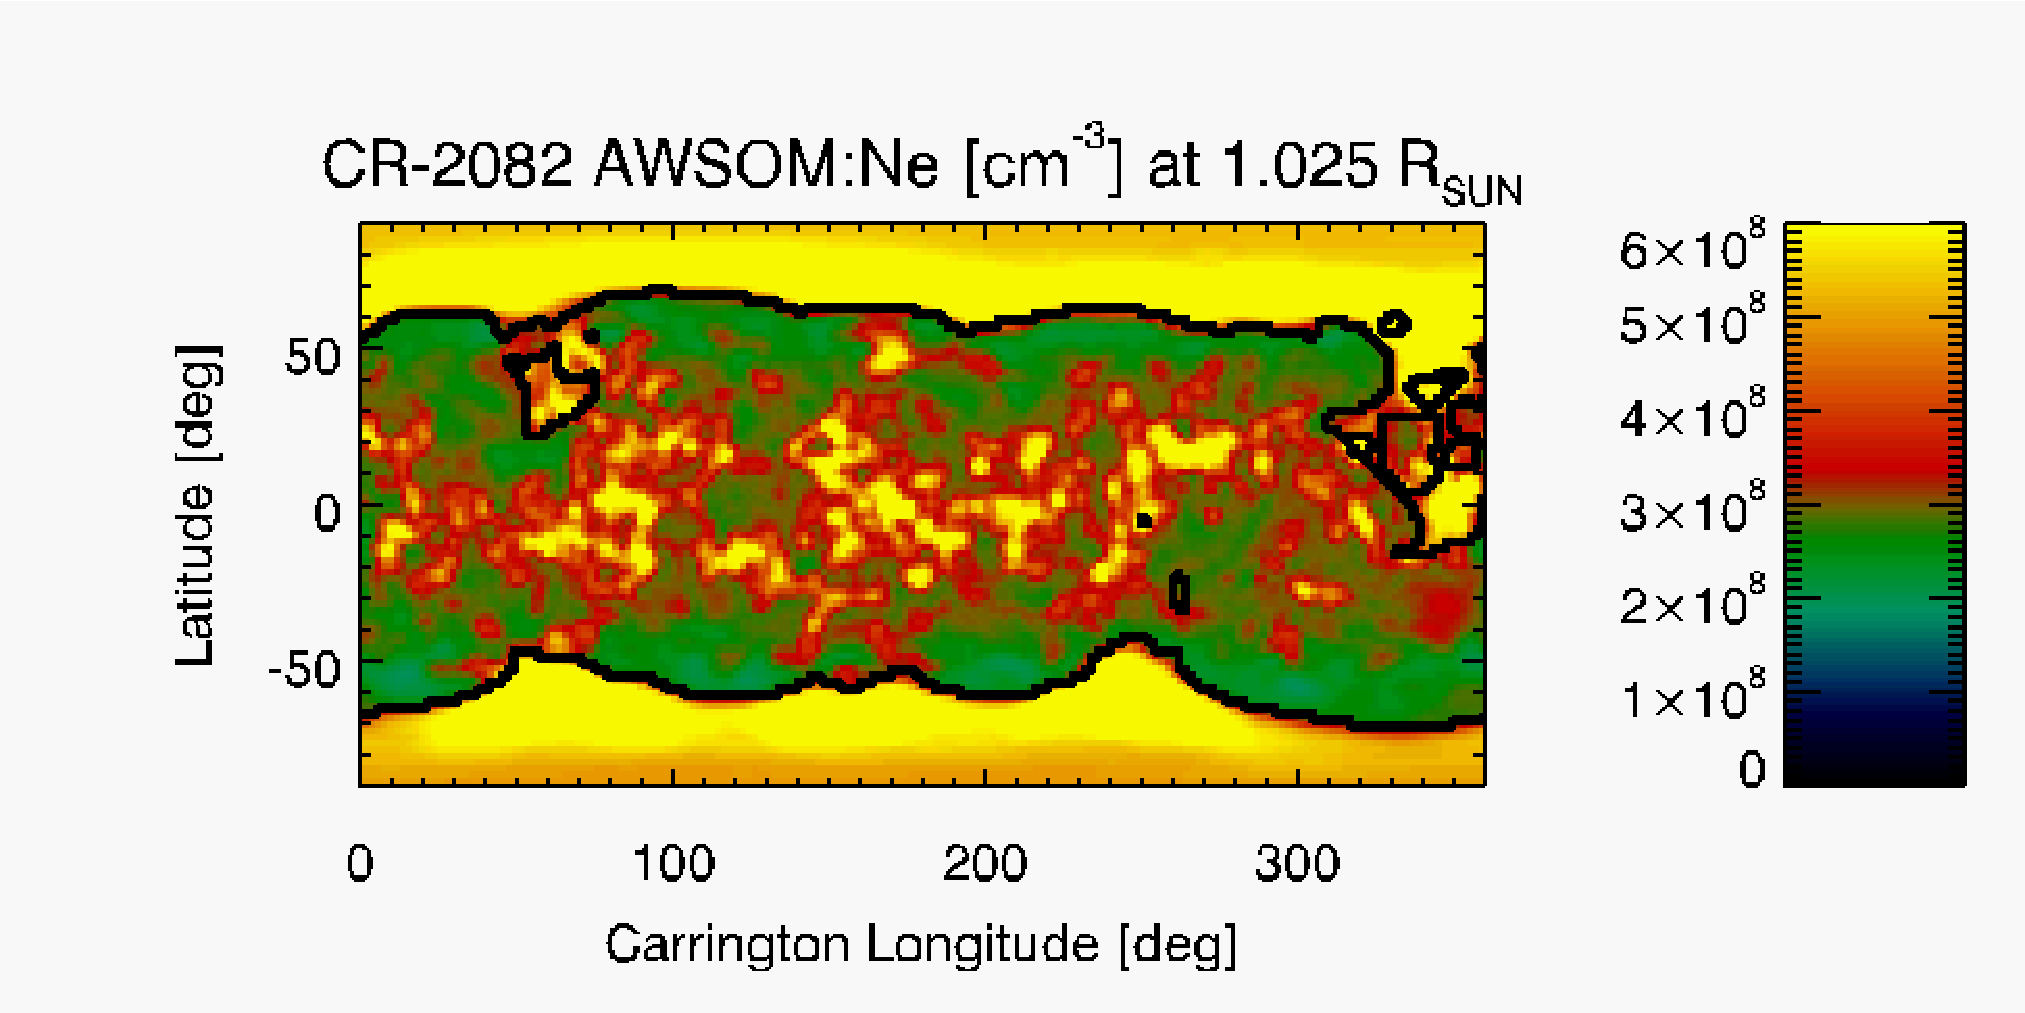
\includegraphics[width=0.495\textwidth]{figs/map_Ne_awsom_2082_185_short_1025_Rsun.pdf}
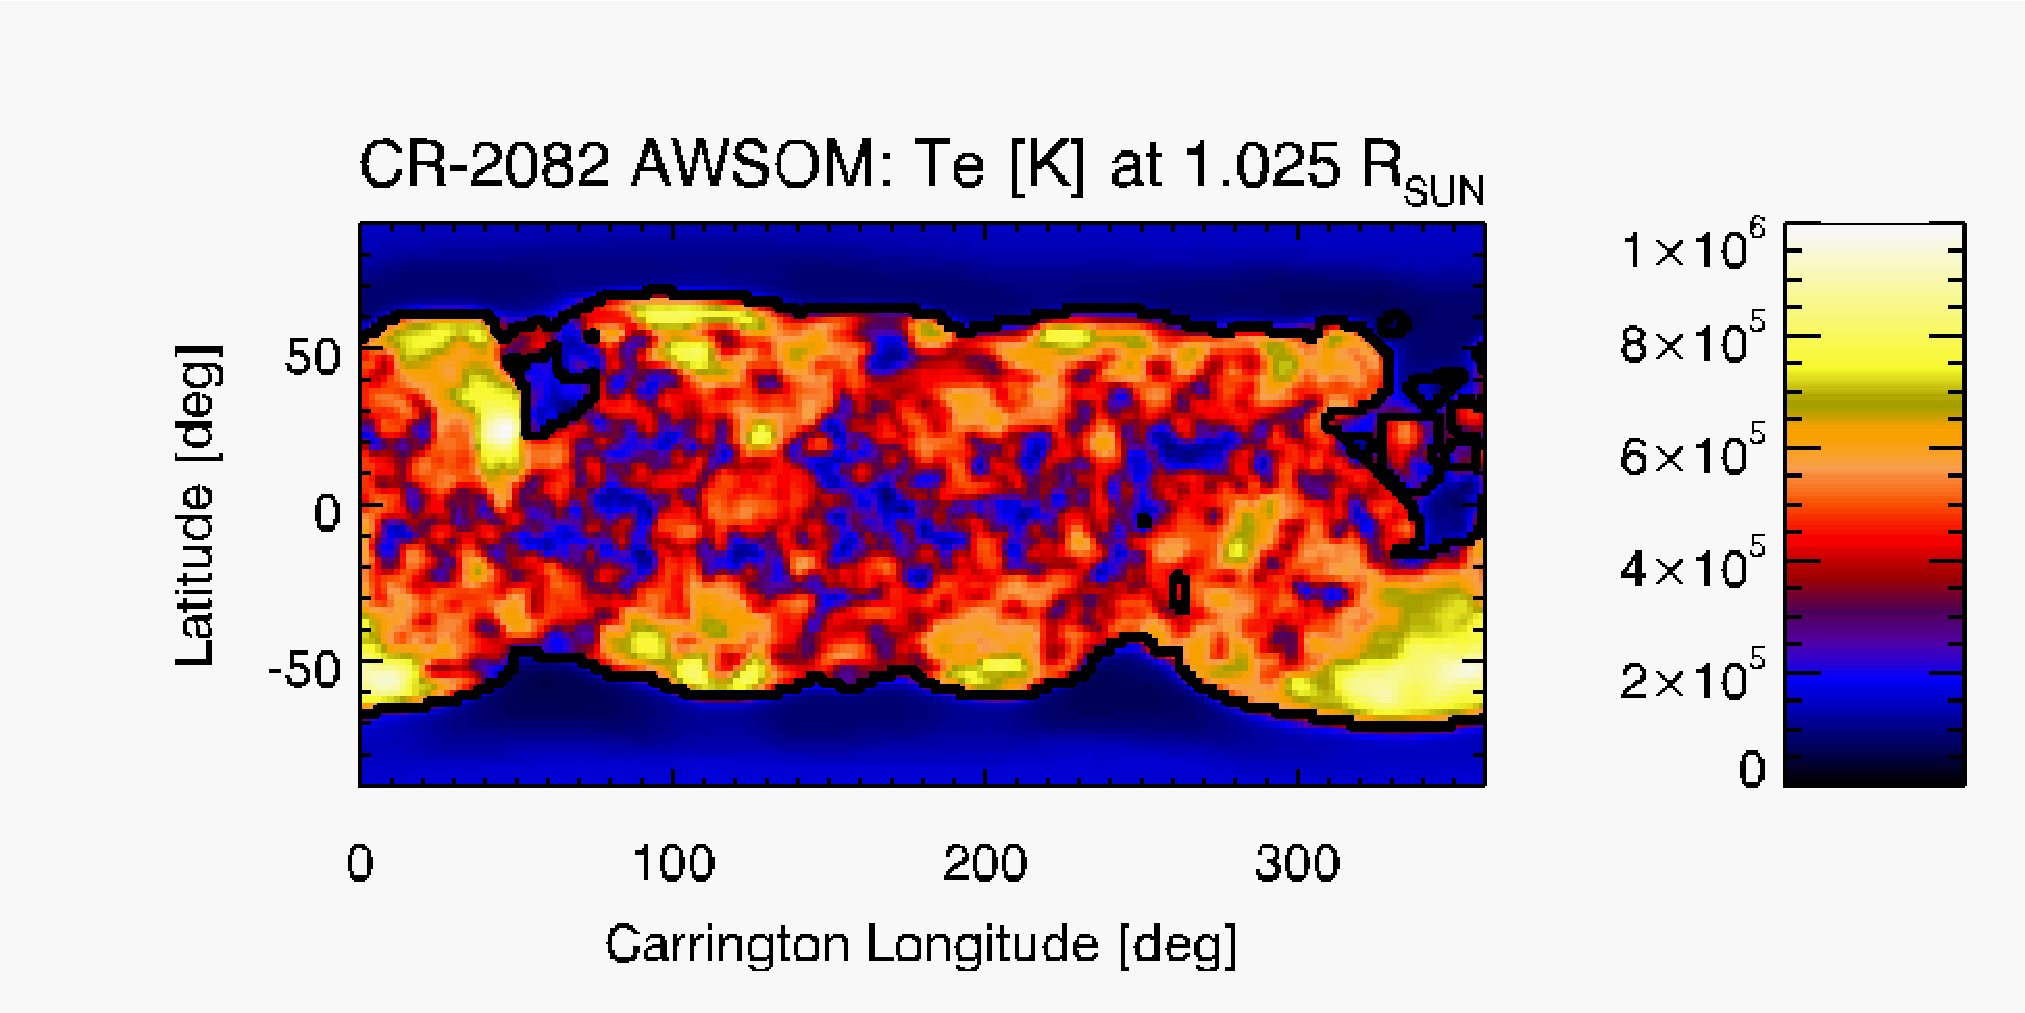
\includegraphics[width=0.495\textwidth]{figs/map_Te_awsom_2082_185_short_1025_Rsun.pdf}
 
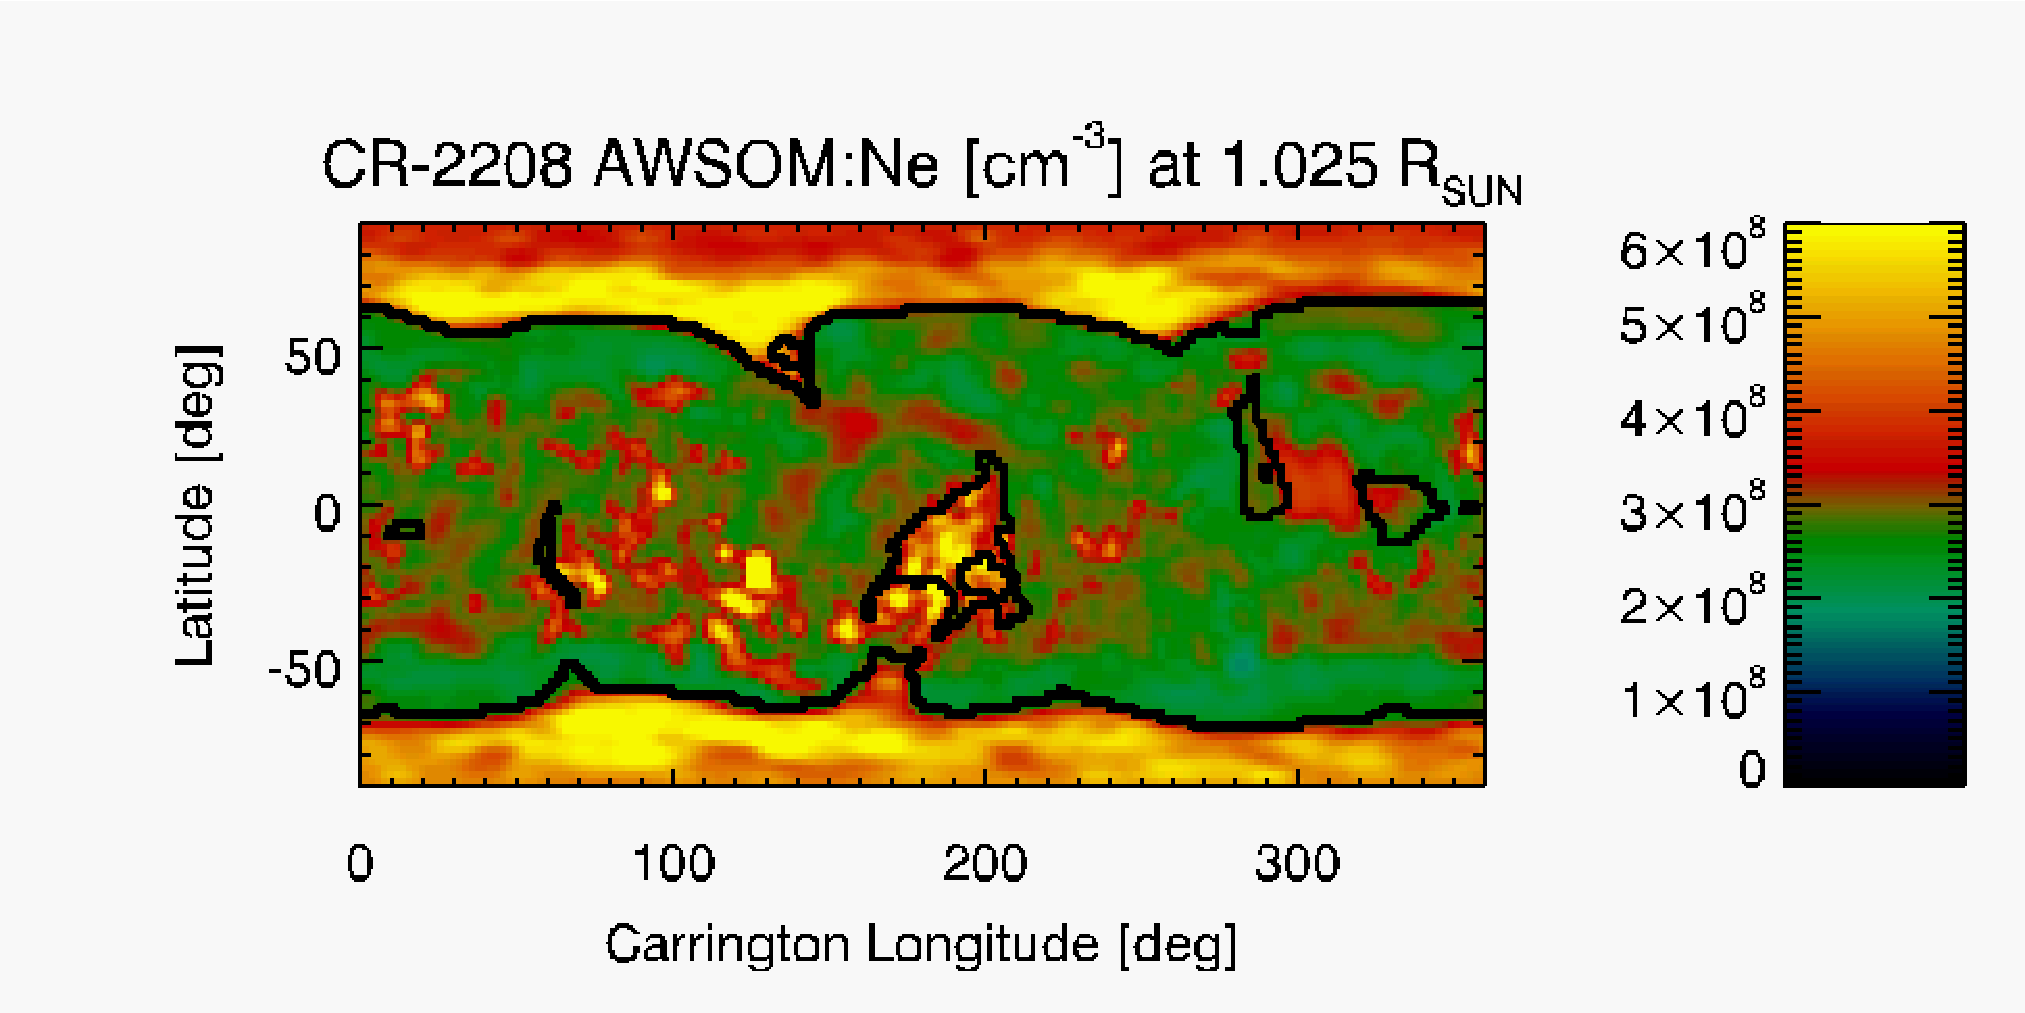
\includegraphics[width=0.495\textwidth]{figs/map_Ne_awsom_2208_185_short_1025_Rsun.pdf}
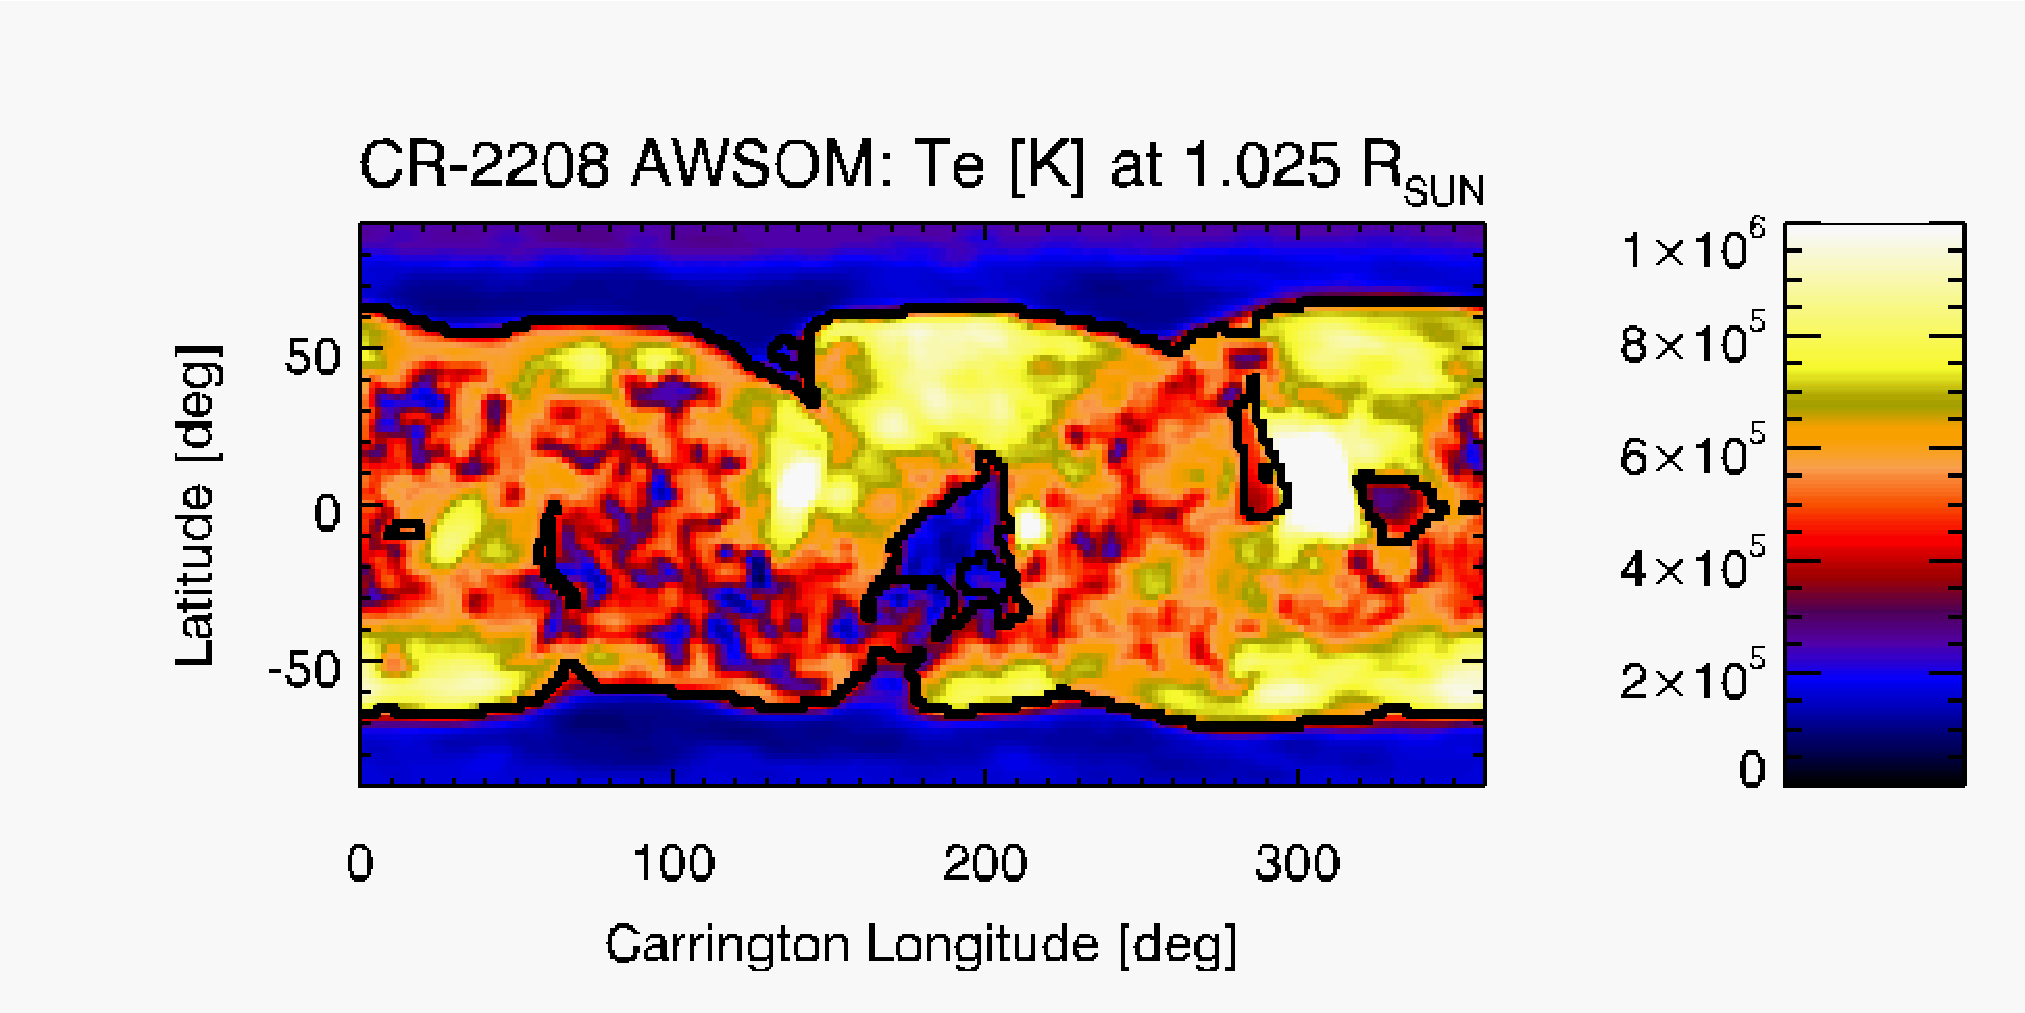
\includegraphics[width=0.495\textwidth]{figs/map_Te_awsom_2208_185_short_1025_Rsun.pdf}

As a result of the former, artifacts introduced by coronal dynamics are mitigated, and as a result of the latter, tomographic reconstructions behave more smoothly close to the radial boundaries of the computational grid when compared to previous reconstructions. 
 
\begin{figure}[h!]
\begin{center}
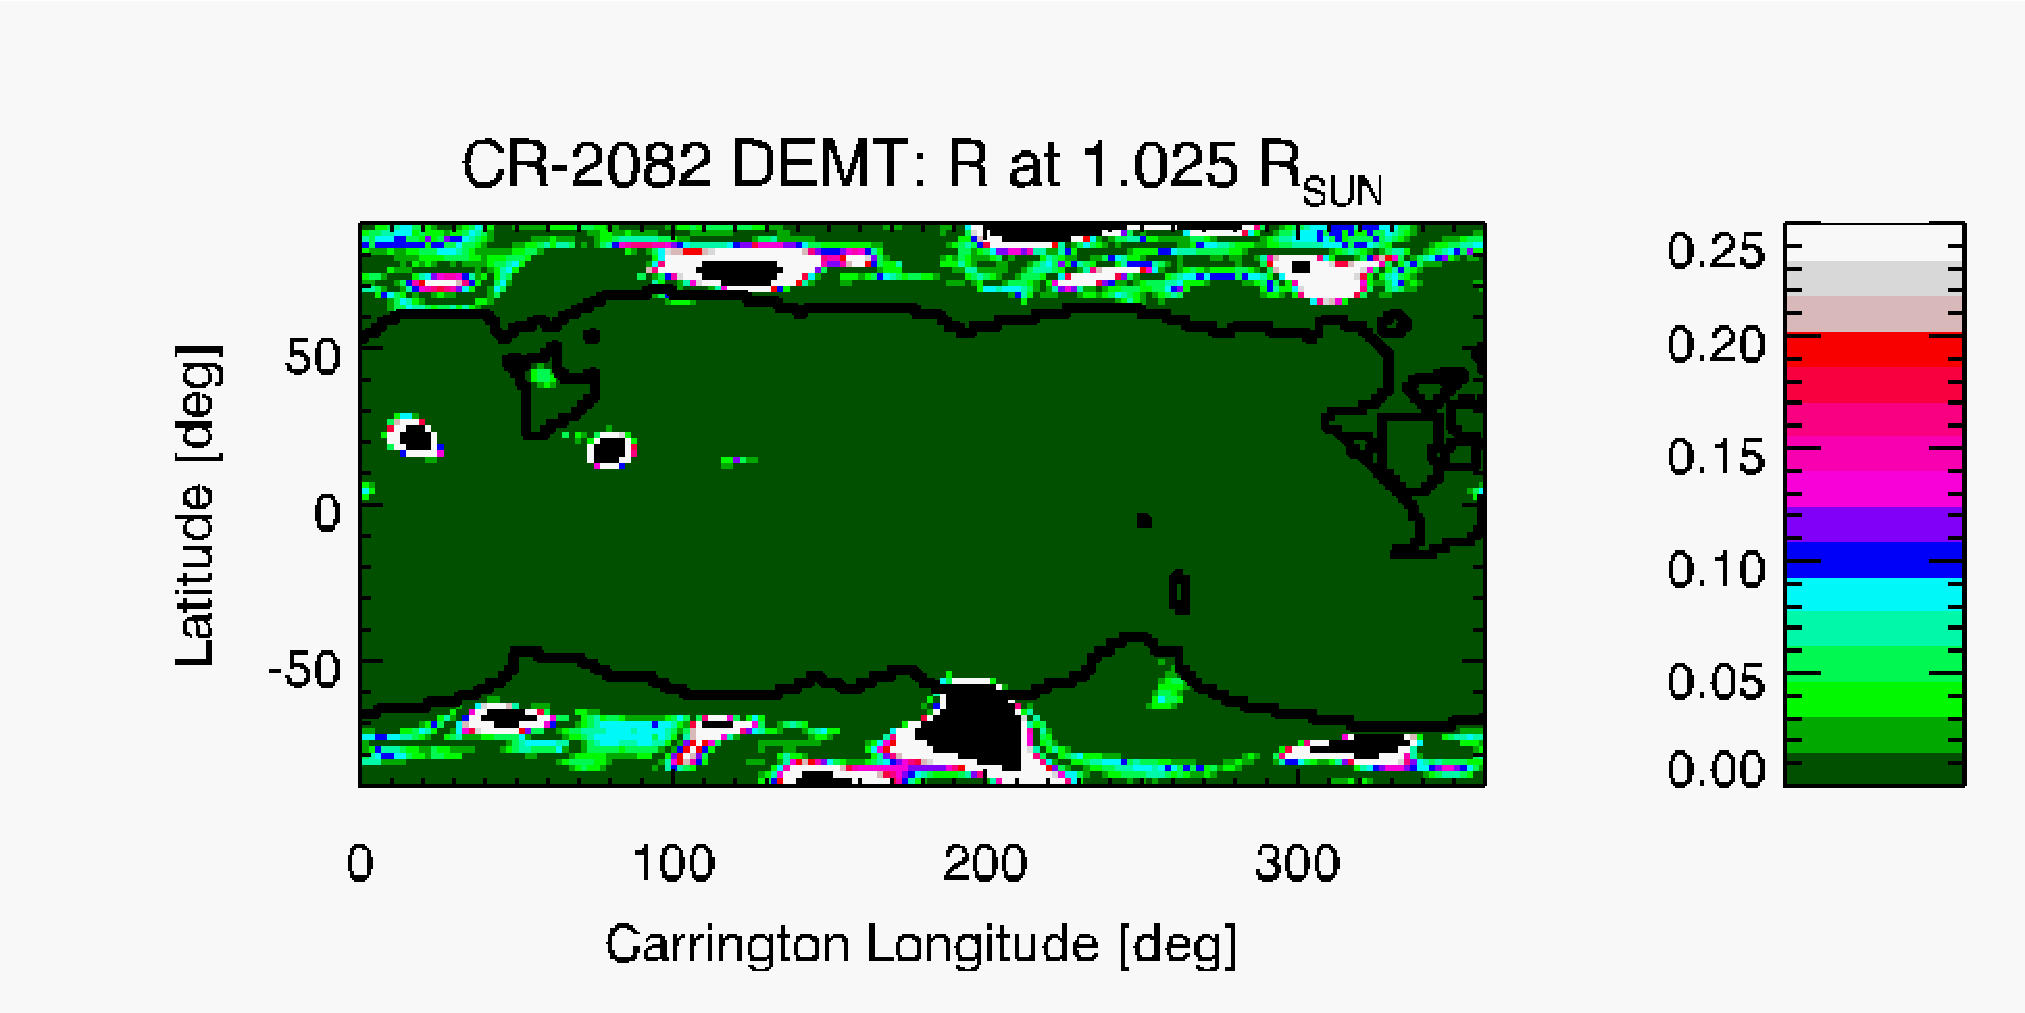
\includegraphics[width=0.495\textwidth]{figs/map_R_CR2082_DEMT-EUVI_behind_H1-L3523_r3d_1025_Rsun.pdf}
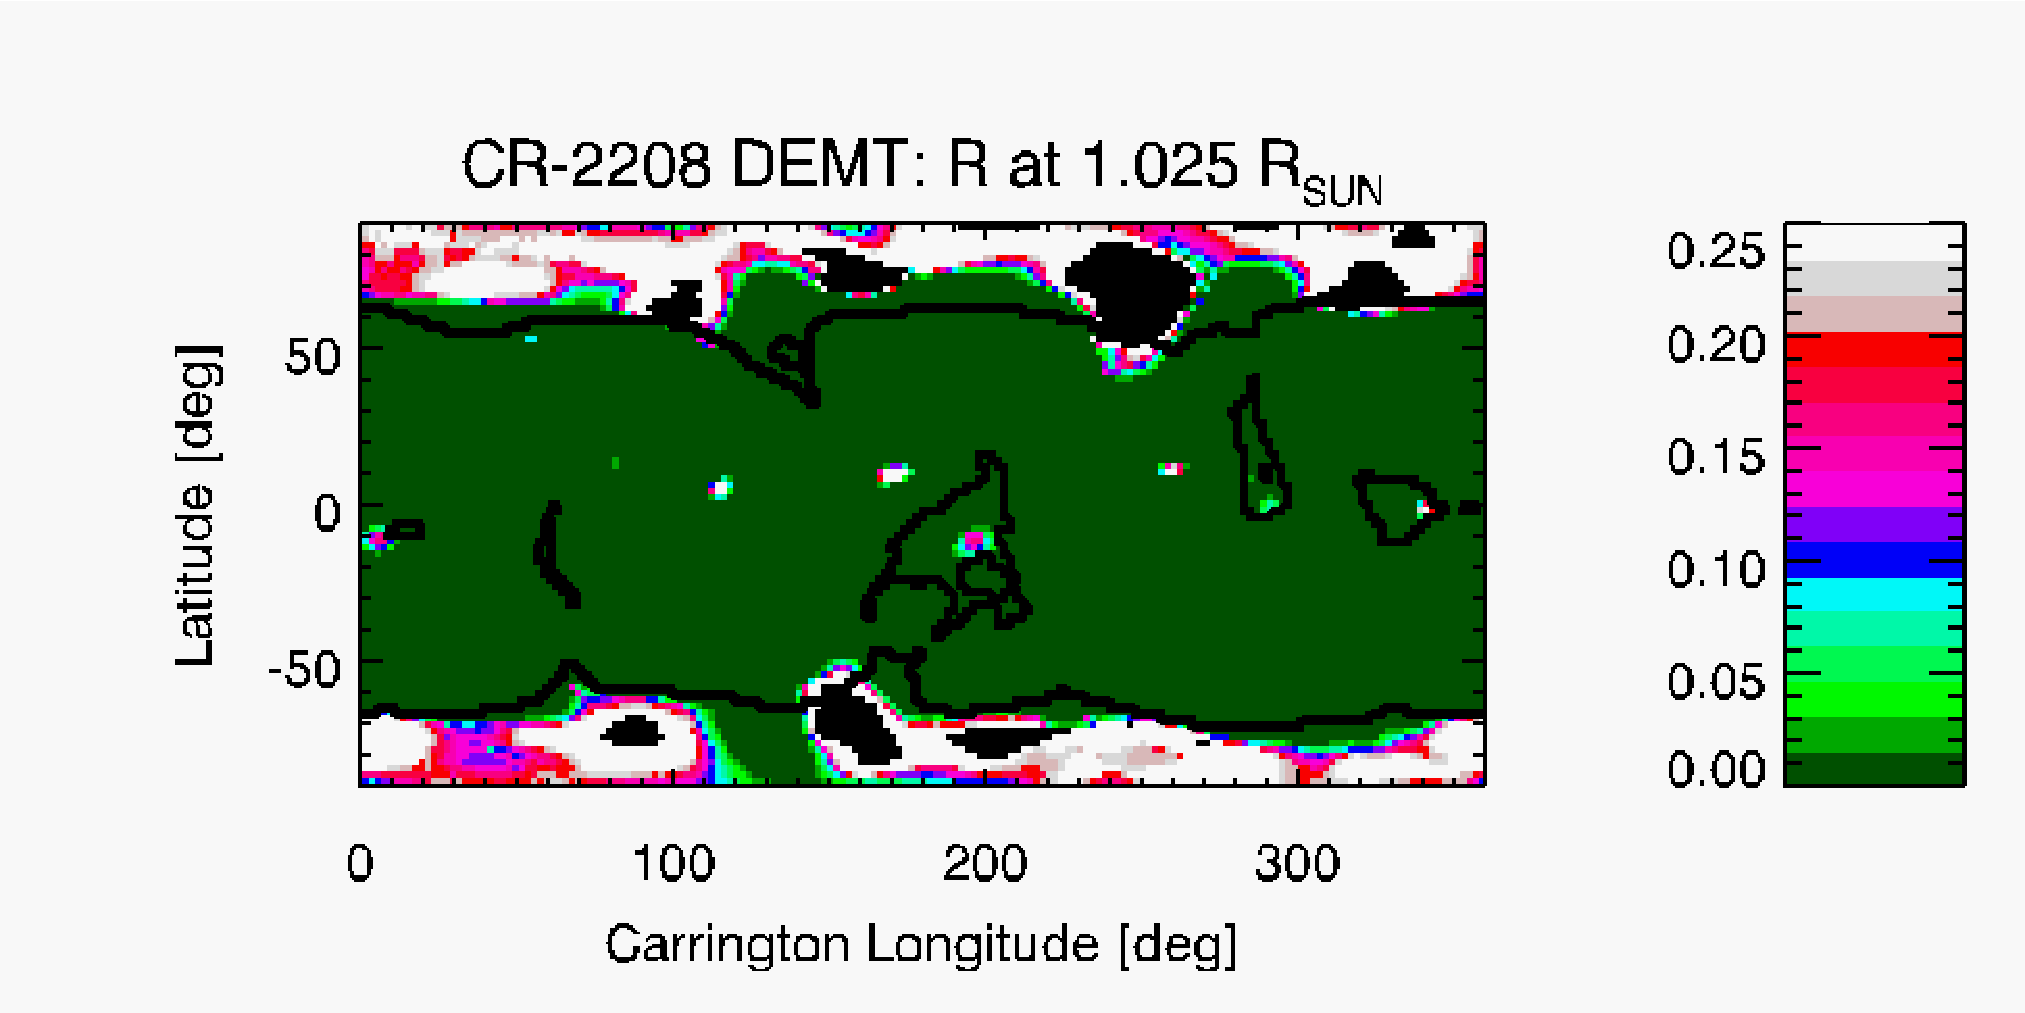
\includegraphics[width=0.495\textwidth]{figs/map_R_CR2208_DEMT-AIA_H1_L522_r3d_1025_Rsun.pdf}
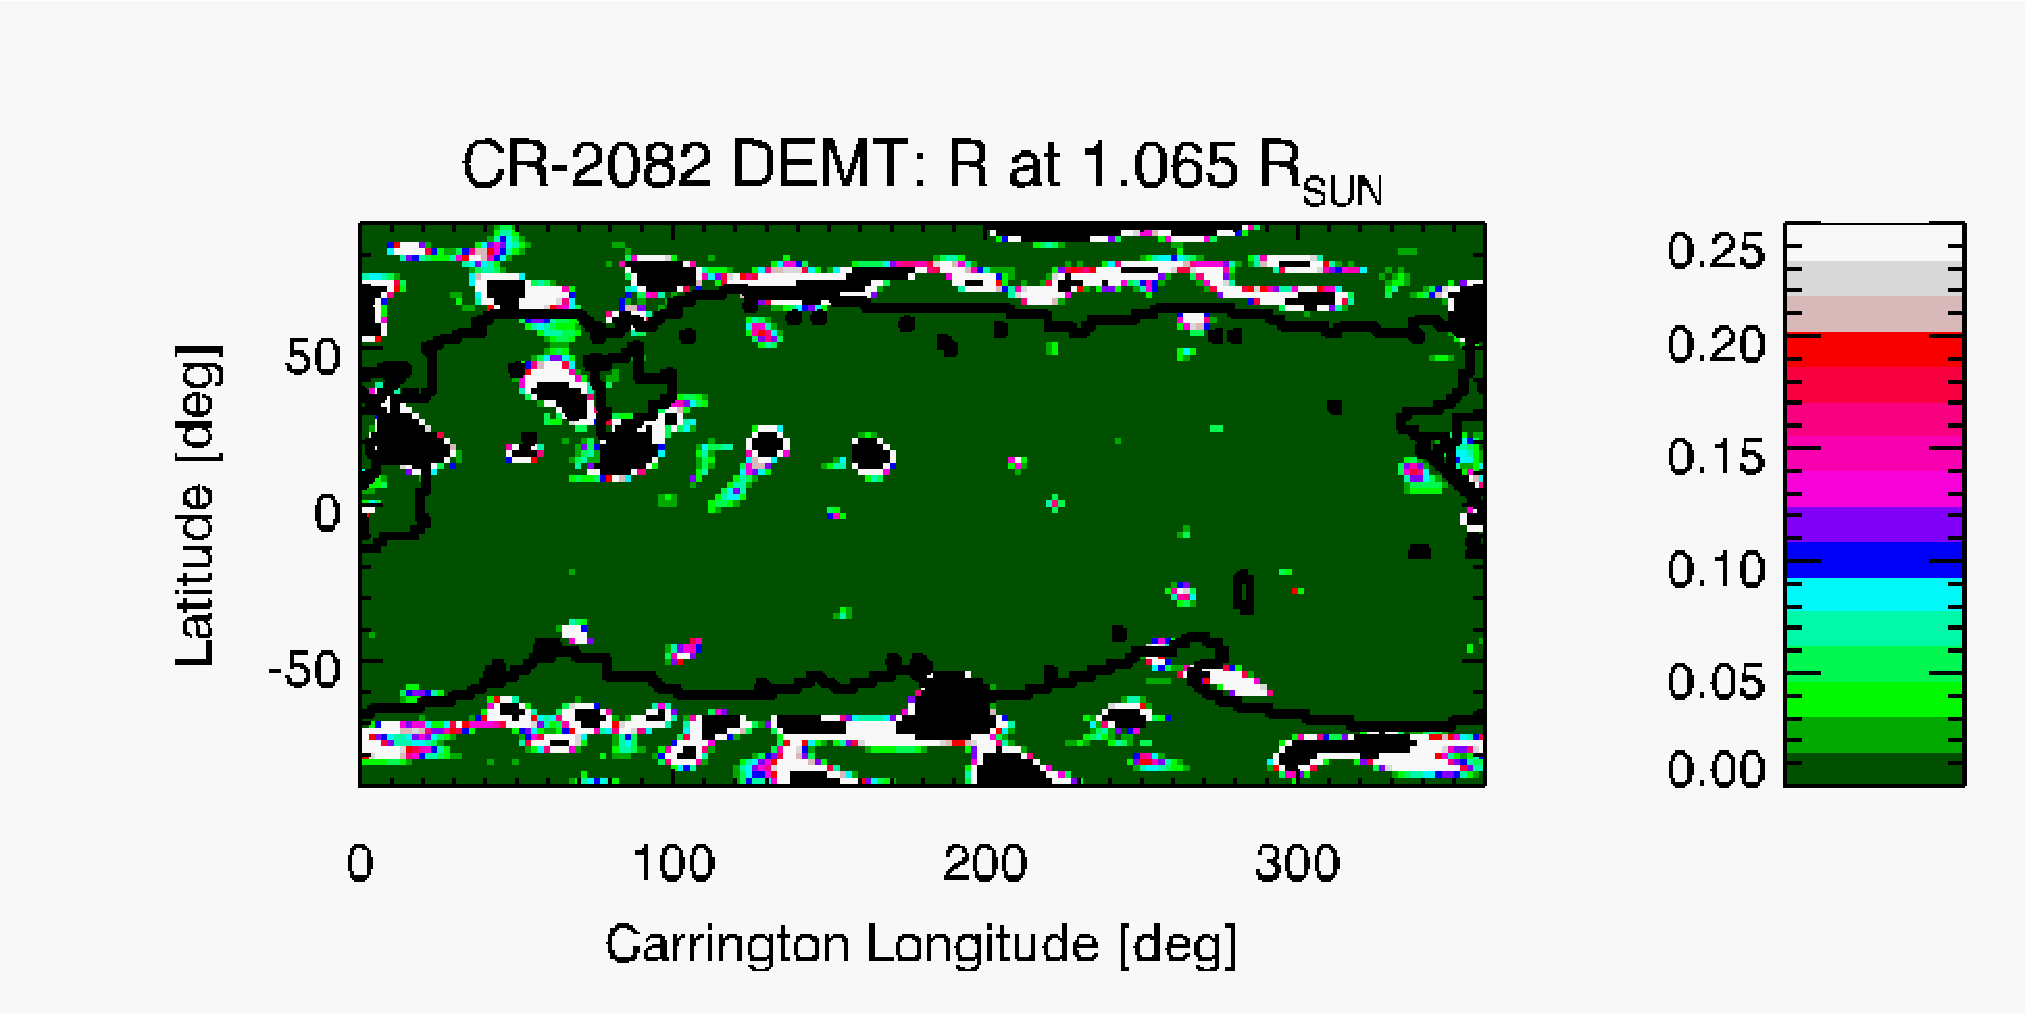
\includegraphics[width=0.495\textwidth]{figs/map_R_CR2082_DEMT-EUVI_behind_H1-L3523_r3d_1065_Rsun.pdf}
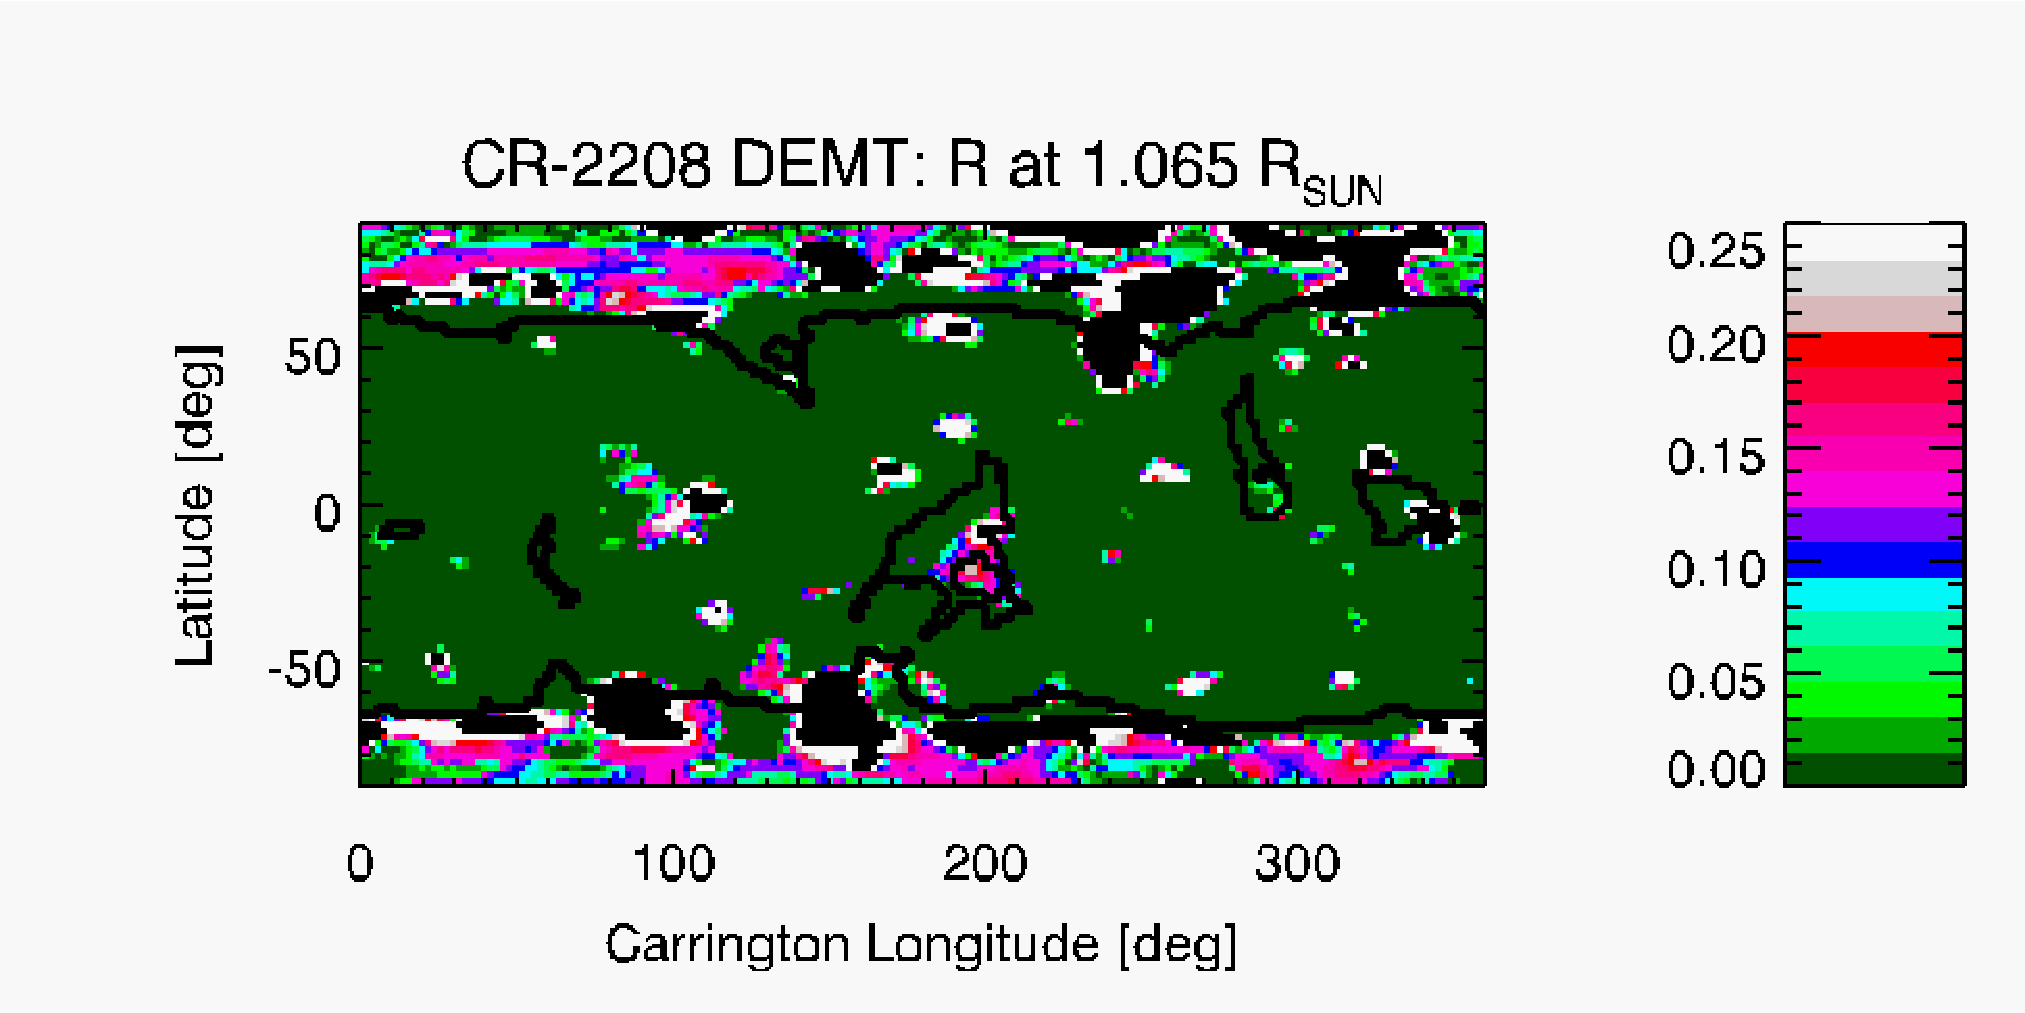
\includegraphics[width=0.495\textwidth]{figs/map_R_CR2208_DEMT-AIA_H1_L522_r3d_1065_Rsun.pdf}
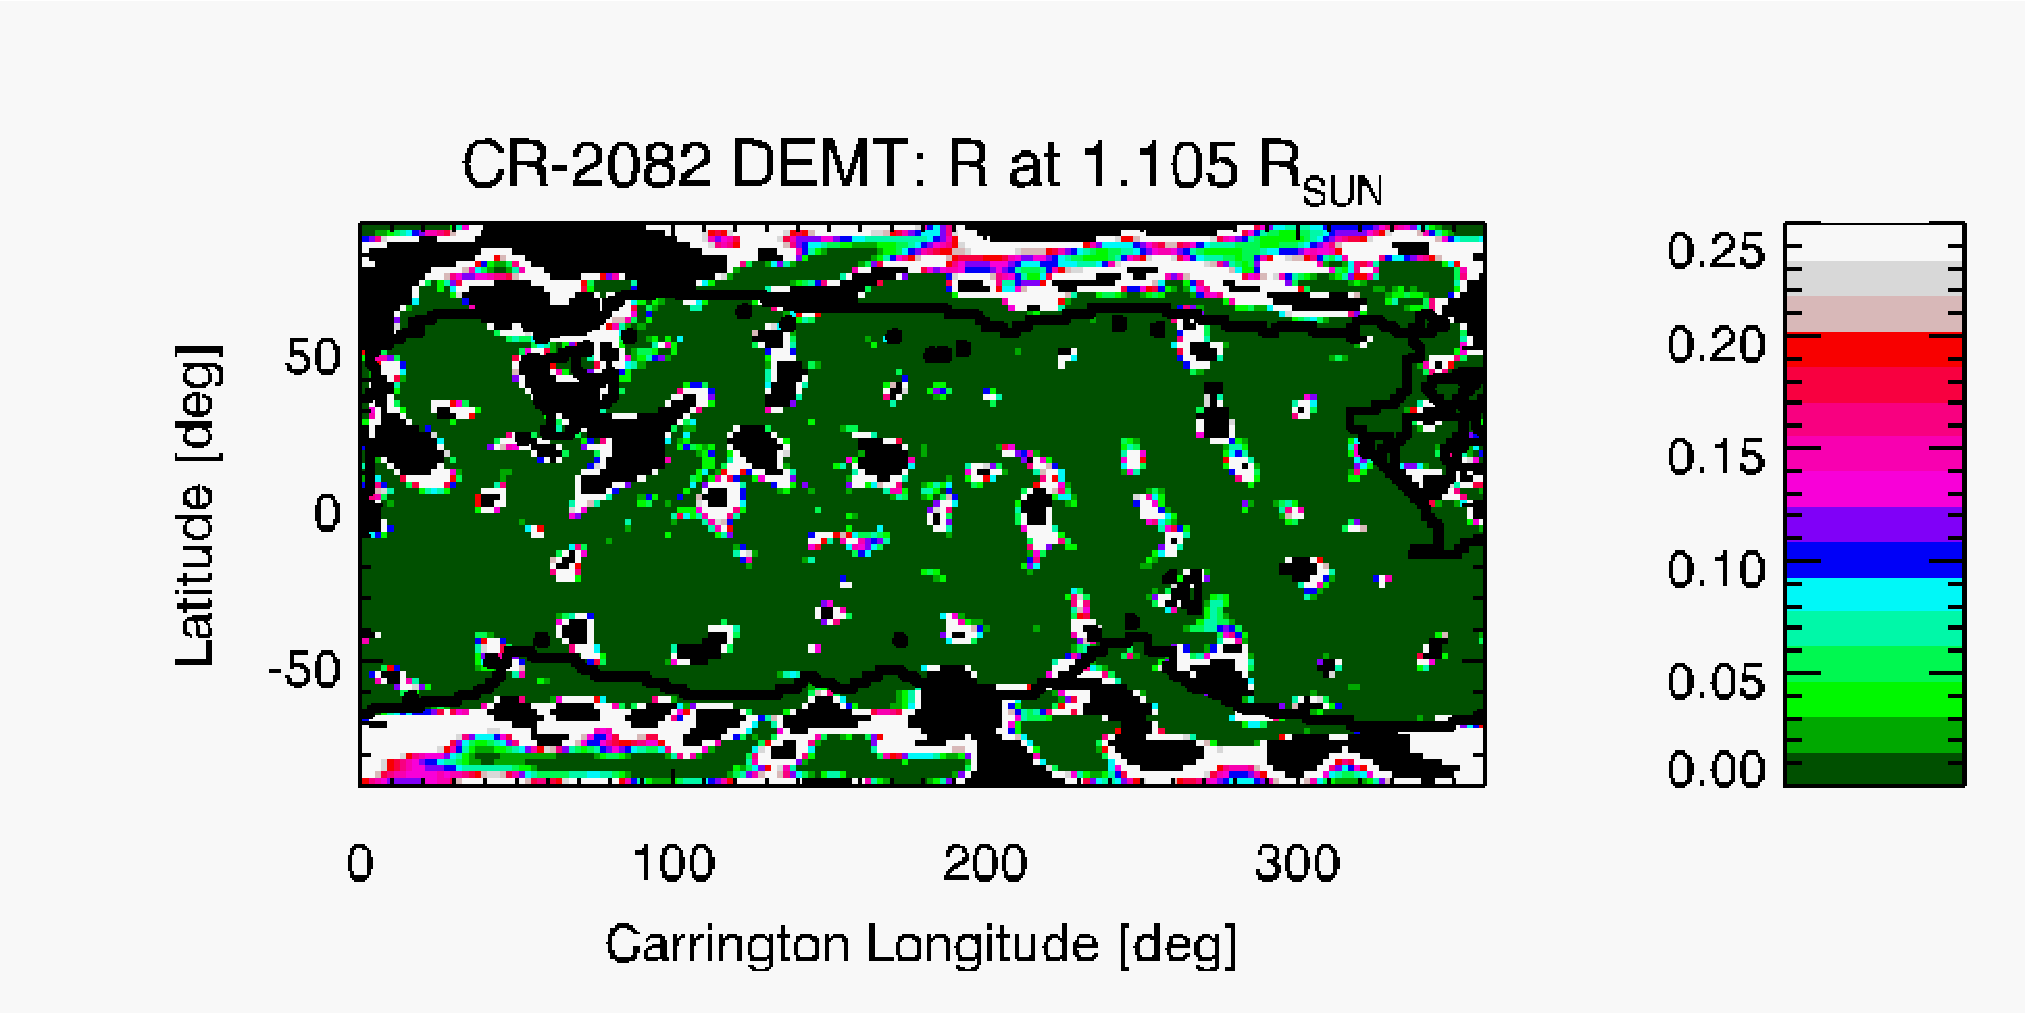
\includegraphics[width=0.495\textwidth]{figs/map_R_CR2082_DEMT-EUVI_behind_H1-L3523_r3d_1105_Rsun.pdf}
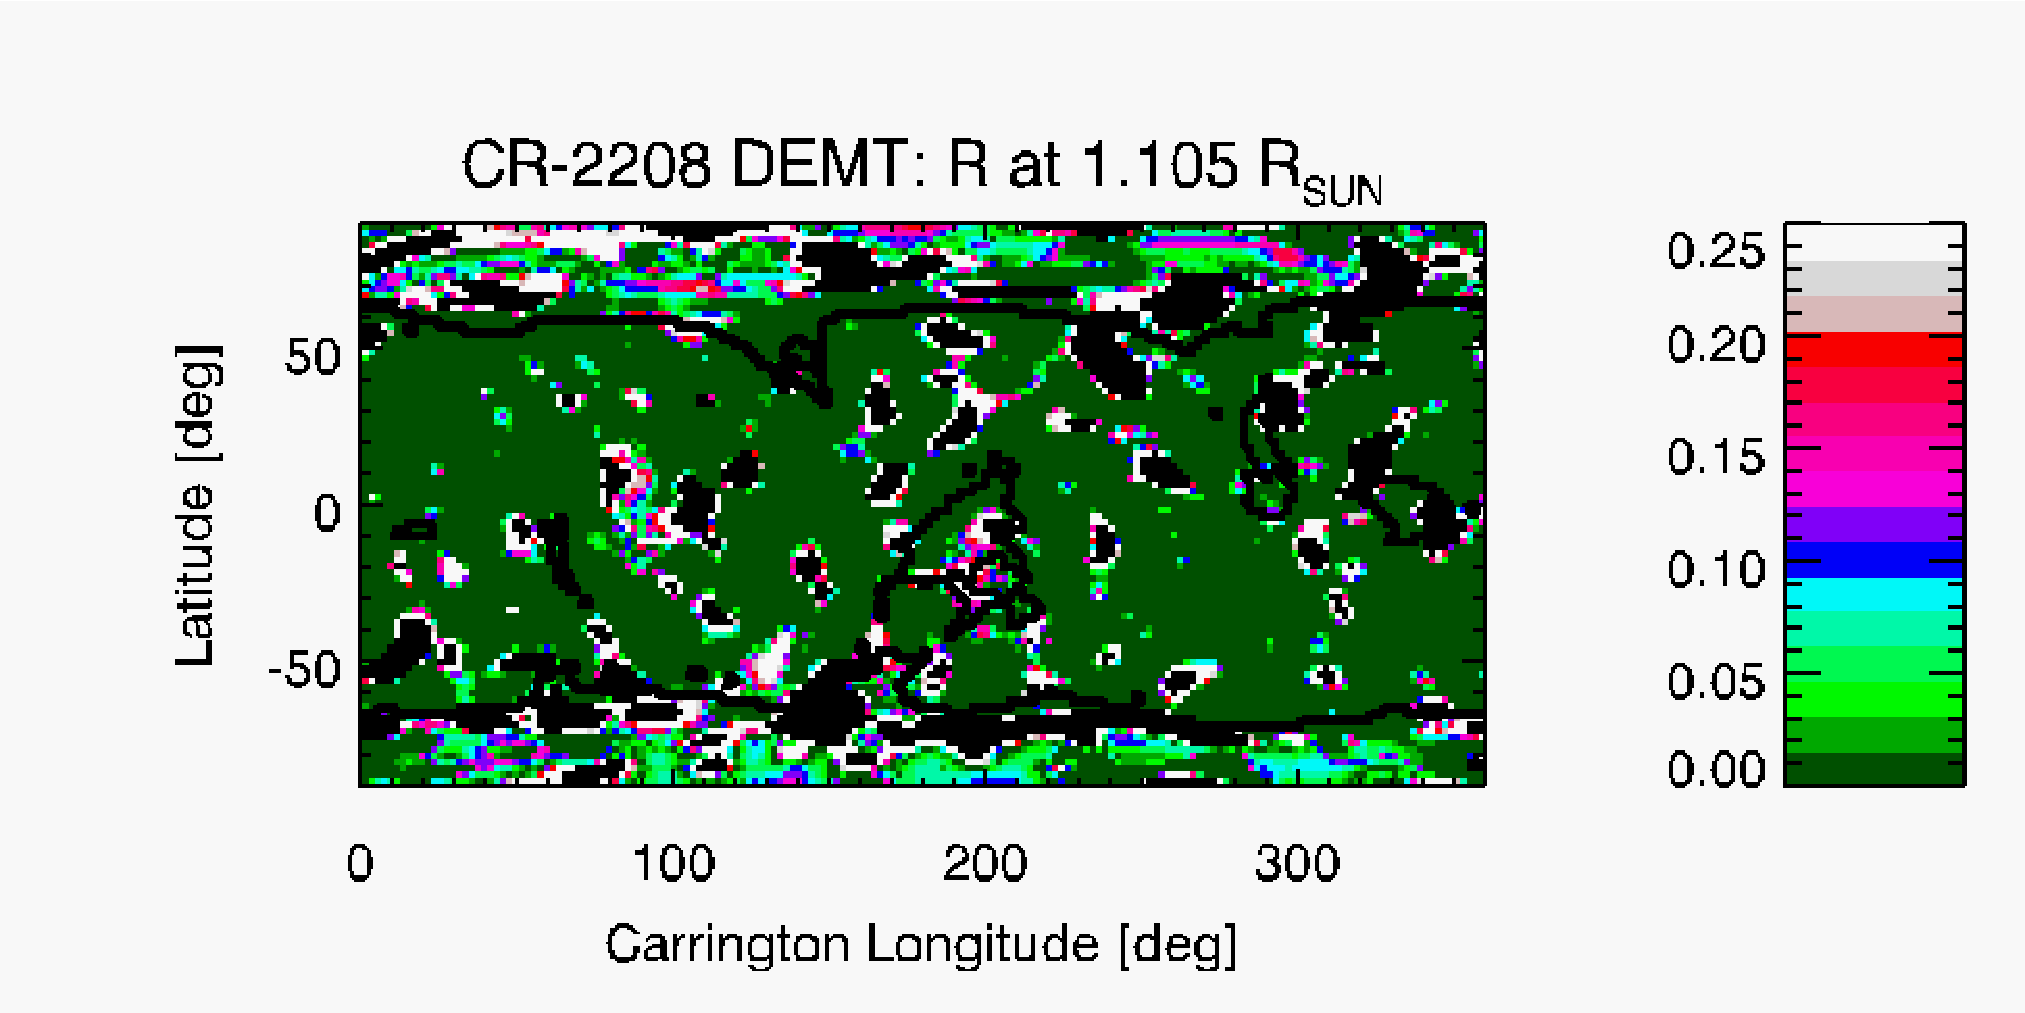
\includegraphics[width=0.495\textwidth]{figs/map_R_CR2208_DEMT-AIA_H1_L522_r3d_1105_Rsun.pdf}
\caption{{Carrington maps of the measure $R$ defined by Equation \ref{R}, for CR-2082 (left panels) and CR-2208 (right panels), at heights $1.025$, $1.065$ and $1.105\,\mrsun$, from top to bottom}. }
\label{carmaps_R_2082_2208}
\end{center}
\end{figure}


{For both rotations, Figure \ref{carmaps_R_2082_2208} shows {latitude-longitude} maps of {the DEMT} measure $R$ defined by Equation \ref{R}, at the same three heights shown in Figures \ref{momento1} and \ref{momento2}.

%\notebyalbert{No comprendo esta frase:} \emph{This classification of types of lines automatically leads to specific regions arranged along all longitudes associated with different thermodynamic, with good symmetry between both hemispheres in both rotations.}

----------------------------------------------------

%\temp{mostrar los gradientes negativos va a ser util en los parrafos posteriores que expliquen porque en las lineas tipo 0 hay valores de $\phi_c$ negativos.} 

%\temp{ Comentar en la discusion el paper de shift y cramer, para decir un poco sobre los down y la incapacidad del modelo en reproducirlos}


----------------------------------------------------

%To establish if the differences in the results between the two rotations are significant, Section \ref{uncertainties} estimates the error bars due the dominating systematic uncertainties.
%\diego{quizas vale la pena introducir alguna comparacion sobre el campo magnetico, veremos como quedan los comentarios de ceci.}
%{Also, within the streamer belt the magnetic field strength is similar in both rotations in the northern hemisphere, while in the southern hemisphere CR-1915 exhibits $10-80\%$ larger values compared to CR-2081, with increasing difference for larger latitudes. In the coronal holes, the magnetic field strength of CR-1915 is much larger than for CR-2081, exhibiting values up to 50\% larger in the northern hemisphere and more than twice larger in the southern hemisphere.}

%Previous works have found magnetic loops which temperature decrease with height, most generally in equatorial latitudes \citep{huang_2012,nuevo_2013}. This type of loops with negative gradients produce a negative conductive flux that contribute to the heating in the corona. In this work, we compute the loop-integrated energy quantities separately in three different populations of loops. 

----------------------------------------------------

%Type 0 loops present slightly larger gradients than type I. Therefore, type 0 present bigger amount, in modulus, of loop-integrated conductive flux. Due conductive flux negative can not be assumed as a loss but it can be contributing to the coronal heating. Thus, to compensate the radiative losses, a lower loop-integrated energy input flux ($\phi_h$) is required.

%We can see, on type 0 loops, a median value of energy input flux for CR2082 twice bigger than CR2208. Also, in both rotations, we observe a negative population of loop integrated energy input flux. This can refer to some loops where loop-integrated radiative flux is too small in comparison with the larger gradients of negative conductive flux, resulting in negative energy input flux. 

%The type I loops show a loop-integrated positive conductive for each loop in both rotations consistent with positive gradients of temperatures. The conductive flux have values around 0.3 $10^{5}[\rm{erg\,sec^{-1}\,cm^{-2}}]$ in both rotations. Similar results have been found for loop-integrated radiative flux and energy input flux for both rotations.

----------------------------------------------------

 with latitudinal gradients of both density and temperature  maximum in the open-close boundary. The open field regions in low latitudes maintain thermodynamic values associated with open regions.} The reconstruction of CR-2082 does not show clear the ARs, while CR-2208 shows a well reconstruction of both AR around latitude-longitud $+5\mdeg$, $140\mdeg$ and $+5\mdeg$, $300\mdeg$. In both rotations the open-closed boundaries derived from the AWSoM model match the shape of the contour levels of both the electron density and the electron temperature.
 
 
 
